% !TeX root = ./main.tex
\documentclass[3p]{elsarticle}

\usepackage{paralist}
\usepackage{lineno,hyperref}
\usepackage{times}
\usepackage{graphicx}
\usepackage{latexsym}
\usepackage{hyperref}
\usepackage{paralist}
\usepackage{ifthen}
%\usepackage{enumitem}
\usepackage{xcolor}
\usepackage{xspace}
\usepackage{amsmath,amssymb}
% \usepackage{algpseudocode}
\usepackage[ruled,linesnumbered]{algorithm2e}
\usepackage{caption}
\usepackage{subcaption}
\usepackage{float}
\usepackage{soul}


\usepackage{lscape}


\definecolor{vuborange}{rgb}{1.0,0.40,0.0}


\newcommand\m[1]{\ensuremath{#1}\xspace}
\newcommand\ltrue{\m{\mathbf{t}}}
\newcommand\lunkn{\m{\mathbf{u}}}
\newcommand\lfalse{\m{\mathbf{f}}}
\newcommand\leqp{\m{\leq_p}}
\newcommand\geqp{\m{\geq_p}}
\newcommand\entails{\m{\models}}
% \newcommand\land{\m{\wedge}}
\newcommand\limplies{\m{\Rightarrow}}
\newcommand\ourtool{\textsc{ZebraTutor}\xspace}
\newcommand\idp{\textsc{IDP}\xspace}
\usepackage{amsthm}
\usepackage{thmtools} 

\newtheorem{thm}{Theorem}
\newtheorem{definition}[thm]{Definition}
\newtheorem{prop}{Property}
\newtheorem{property}[prop]{Property}
\newtheorem{ex}{Example}
\newtheorem{example}[ex]{Example}
\newcommand\xxx{\m{\overline{x}}}
\newcommand\ddd{\m{\overline{d}}}

%To easily allow for saving space
\newcommand{\myparagraph}[1]{\subsection{#1}}

\newcommand\allconstraints{\m{T}}
\modulolinenumbers[5]

\journal{Journal of Artificial Intelligence}

%% `Elsevier LaTeX' style
\bibliographystyle{elsarticle-num}
%%%%%%%%%%%%%%%%%%%%%%%
%% `User comments`
\newcommand\comment[1]{\marginpar{\tiny #1}}
\renewcommand\comment[1]{#1}
\newcommand{\bart}[1]{{\comment{\color{red}\textsc{BB:}#1}}}
\newcommand{\tias}[1]{{\comment{\color{blue}\textsc{TG:}#1}}}
\newcommand{\emilio}[1]{{\comment{\color{red}\textsc{EG:}#1}}}
\newcommand{\todelete}[1]{{\comment{\color{red}\st{#1}}}}
\newcommand{\todo}[1]{{\comment{\color{red}\textsc{TODO:}#1}}}
\newcommand\ignore[1]{}
\newcommand{\toprule}{}
\newcommand{\midrule}{\hline}
\newcommand{\bottomrule}{}

% comment out for removing the comments
% \renewcommand\comment[1]{}

%%%%%%%%%%%%%%%%%%%%%%%

\begin{document}


\begin{frontmatter}

\title{A framework for step-wise explaining how to solve constraint satisfaction problems}
%\tnotetext[mytitlenote]{Fully documented templates are available in the elsarticle package on \href{http://www.ctan.org/tex-archive/macros/latex/contrib/elsarticle}{CTAN}.}

%% Group authors per affiliation:
\author[mymainaddress]{Bart Bogaerts, Emilio Gamba, Tias Guns}
\address{Vrije Universiteit Brussel, Pleinlaan 2, 1050 Brussel, Belgium}
\ead{\{firstname.lastname\}@vub.be}

\begin{abstract}
We explore the problem of step-wise explaining how to solve constraint satisfaction problems, with a use case on logic grid puzzles.
More specifically, we study the problem of explaining the inference steps that one can take during propagation, in a way that is easy to interpret for a person.
Thereby, we aim to give the constraint solver explainable agency, which can help in building trust in the solver by being able to understand and even learn from the explanations.
The main challenge is that of finding a sequence of \textit{simple} explanations, where each explanation should aim to be as cognitively easy as possible for a human to verify and understand. 
This contrasts with the arbitrary combination of facts and constraints that the solver may use when propagating.
We propose the use of a cost function to quantify how simple an individual explanation of an inference step is, and identify the explanation-production problem of finding the best sequence of explanations of a CSP. 
Our approach is agnostic of the underlying constraint propagation mechanisms, and can provide explanations even for inference steps resulting from combinations of constraints. 
In case multiple constraints are involved, we also develop a mechanism that allows to break the most difficult steps up and thus gives the user the ability to \emph{zoom in} on specific parts of the explanation. 
Our proposed algorithm iteratively constructs the explanation sequence by using an optimistic estimate of the cost function to guide the search for the best explanation at each step.
Our experiments on logic grid puzzles show the feasibility of the approach in terms of the quality of the individual explanations and the resulting explanation sequences obtained.
\end{abstract}

\begin{keyword}
Artificial Intelligence \sep Constraint Solving \sep Explanation
%\texttt{elsarticle.cls}\sep \LaTeX\sep Elsevier \sep template
%\MSC[2010] 00-01\sep  99-00
\end{keyword}

\end{frontmatter}

\linenumbers

\section{Introduction}\label{sec:intro}
Need for explanations of reasoning systems

Shallow related work on quickxplain, 'explanations' in search, etc.

HolyGrail challenge and related work

Difference automated reasoning and human reasoning, measuring cognitive load

challenge 1: abstraction in self-contained reasoning step

challenge 2: ordering

challenge 3: computation efficiency

Contributions: (eerste aanzet!!!)

\begin{itemize}
	\item Formalize the problem of finding good ordering of self-contained reasoning steps
	\item Investigate different interpretations of good ordering and self-contained
	\item Propose algorithms to approximate the ???some hardness result??? problem of finding the best ordering
	\item Experimentally demonstrate the quality and feasibility of the approach
\end{itemize}


\bart{Mention running example? Mention that this is a very hard puzzle (80 people at an AI conference received it; 4 solved it; many more tried)? }


\section{Related work}\label{sec:related-work}
This research fits within the general topic of Explainable Agency~\cite{langley2017explainable}, whereby in order for people to trust autonomous agents, the latter must be able to explain their decisions and the reasoning that produced their choices. 
For example, explainable planning~\cite{fox2017explainable} is concerned with building planning systems that can explain their own behaviour. This includes answering queries such as ``why did the system (not) make a certain decision'', ``why is this the best decision'', etc. In contrast to explainable machine learning research, in explainable planning one can make use of the explicit \textit{model-based representation} over which the reasoning happens. Likewise, we will make use of the constraint specification available to constraint solvers. %, and focus on providing explanations of propagation steps in an interpretable way.

Explanation of constraint satisfaction problems has been studied mostly in the context of overconstrained problems. 
The goal then is to find which constraints conflict with each other. The QuickXplain method \cite{junker2001quickxplain} for example uses a dichotomic approach that recursively partitions the constraints to find a minimal conflict set. This is also known as the Minimum Unsat Subset (MUS) problem or Minimal Unsat Core extraction~\cite{marques2010minimal}. Many algorithm exist for finding a MUS or enumerating all MUS's~\cite{marques2010minimal}. We will use MUS extraction for finding a minimal explanation of an individual inference step.

Our work is inspired by the holy grail challenge at CP'2019, which in turn has its roots in earlier work of E.~Freuder on inference-based explanations \cite{sqalli1996inference}. In that work, the authors investigate logic grid puzzles and develop a number of problem-specific inference rules that allow solving such puzzles without search. These inference rules are equipped with explanation templates such that each propagation event of an inference rule also has a templated explanation, and hence an explanation of the solution process is obtained. We point out that the more complex inference rules (NCC and GNCC) are in inference rules over hard-coded combinations of (in)equality constraints. In contrast, our proposed method works for any type of constraint and any combination of constraints, and automatically infers a minimal set of facts and constraints that explain an inference step, without using any problem-specific knowledge. %\bart{can they explain the pasta puzzle? Probably not!} I would expect not: that combination not hard-coded

%DUPLICATE Our work is inspired by the holy grail challenge at CP'2019, which in turn has its roots in earlier work of E. Freuder on inference-based explanations \cite{sqalli1996inference}. In that work, the authors look at logic grid puzzles and develop a number of problem-specific inference rules that allow solving such puzzles without search. These inference rules are equiped with explanation templates such that each propagation event of an inference rule also has a templated explanation, and hence an explanation of the solution process is obtained. We remark that the more complex inference rules (NCC and GNCC) are over hard-coded combinations of (in)equality constraints. In contrast, our proposed method works for any type of constraint and any combination of constraints, and automatically infers a minimal set of facts and constraints that explain a small inference step, without using any problem-specific knowledge.
%Explanation of constraint satisfaction problems has been studied mostly in the context of overconstrained problems. The goal is to find what constraints conflict with each other. 
%The QuickXplain method \cite{junker2001quickxplain} for example uses a dichotomic approach that recursively partitions the constraints to find a minimal conflict set. 
%This is also known as the Minimum Unsat Subset (MUS) problem or Minimal Unsat Core extraction~\cite{marques2010minimal}. Many algorithm exist for finding a MUS or enumerating all MUS's~\cite{marques2010minimal}. We will use MUS extraction for finding a minimal explanation of an individual inference step.


There is a rich literature on automated and interactive theorem proving, recently focussing on providing proofs that are understandable for humans \cite{Ganesalingam2017} and, e.g.,  on teaching humans -- using interaction with theorem provers -- how to craft mathematical proofs  \cite{DBLP:conf/icml/YangD19}. 
Our work fits into this line of research since our generated explanations can also be seen as proofs, but in the setting of finite-domain constraint solving.

% Our work also fits within the general topic of Explainable Agency~\cite{langley2017explainable}, whereby in order for people to trust autonomous agents, the latter must be able to explain their decisions and the reasoning that produced their choices. 
% For example, explainable planning~\cite{fox2017explainable} is concerned with building planning systems that can explain their own behaviour. This includes answering queries such as ``why did the system (not) make a decision'', ``why is this the best decision'' etc. In contrast to explainable machine learning research, in explainable planning one can make use of the explicit \textit{model-based representation} over which the reasoning happens. Likewise, we will make use of the constraint specification available to constraint solvers, and focus on providing explanations of propagation steps in an interpretable way.


\todo{CHECK THIS OUT (reviewer comment):
At a high-level, there seems to be connection to other approaches to explanation. For instance, in the context of decision-aiding, this sort of step-wise explanations have been advocated, with similar concerns it seems regarding the definition of generic complexity functions:
- Belahcene et al. Explaining robust additive utility models by sequences of preference swaps. Theory and Decision, 2017
}


\section{Background}\label{sec:background}\label{sec:prelims}
\textbf{Logic grid puzzles.}
While our proposed method is applicable to constraint satisfaction problems in general, we use \textit{logic grid puzzles} as example domain, as it requires no expert knowledge to understand.

A logic grid puzzle (also known as Zebra puzzle or Einstein puzzle) consists of natural language sentences (from hereon referred to as ``clues'') over a set of \emph{entities} occurring in those sentences. 
For instance, our running example in Figure~\ref{fig:zebrascreen} contains as second clue ``The person who chose arrabiata sauce is either Angie or Elisa'' and (among others) entities ``arrabiata sauce'', ``Angie'' and ``Elisa''. 

The set of entities is sometimes left implicit if it can be derived from the clues, but often it is given in the form of a grid. Furthermore, in such a puzzle the set of entities is partitioned into equally-sized groups (corresponding to \emph{types}); in our example, ``person'' and ``sauce'' are two such types. 
% 
The goal of the puzzle is to find relations between each two types such that
\begin{compactitem}
	\item each clue is respected, 
	\item each entity of one type is matched with exactly one entity of the second type, e.g., each person chose exactly one sauce and each sauce is linked to one person (this type of constraint will be referred to as \emph{bijectivity}), and 
	\item the relations are logically linked, e.g., if Angie chose arrabiata sauce and arrabiata sauce was paired with farfalle, then Angie must also have eaten farfalle (from now on called \emph{transitivity}). 
\end{compactitem}
In Section \ref{sec:holistic} we explain how we obtain a vocabulary and first-order theory in a mostly automated way from the clues. The result is a vocabulary with types corresponding to the groups of entities in the clues, and the names and types of the binary relations to find (e.g \textit{chose(person, sauce)}, \textit{paired(sauce, pasta)}, \textit{eaten(person, pasta)});
%We furthermore assume that the interpretation of the types is fixed (and hence all interpretations agree on this). 
as well as constraints (first-order sentences) corresponding to the clues, and the bijectivity and transitivity constraints. Let $T_P$ be a theory containing all of these constraints for a given puzzle $P$.

Our running example is a puzzle about people having dinner in a restaurant and ordering different types of pasta. It is the hardest logic grid puzzle we encountered (as a reference, at a recent AI conference, when presenting our tool \cite{DBLP:conf/bnaic/ClaesBCGG19}, only four out of 80 researchers who tried managed to solve it).    
The entire puzzle can be seen in Figure \ref{fig:zebrascreen}; the full final explanation generated for it can be found at \url{http://bartbog.github.io/zebra/pasta}.
% Dout of  and its final produced explanation still contains some challenging steps. 

\myparagraph{Typed first-order logic.}
Our constraint solving method is based on \emph{typed first-order logic}. %, with links to \emph{typed second-order logic}.
Part of the input is a logical vocabulary consisting of a set of type symbols, (typed) constant symbols, and (typed) relation symbols with associated type signature (i.e., each relation symbol is typed $T_1\times \dots \times T_n$ with $T_i$ types).\footnote{We here omit function symbols since they are not used in this paper.} For example, type \textit{person} with constant symbol \textit{Angie} of type \textit{person} and a relation \textit{chose(.,.)} with signature \textit{person $\times$ sauce}.


A \emph{first-order theory} is a set of sentences (well-formed variable-free first-order formulas in which each quantified variable has an associated type), also referred to as constraints.
Since we work in a fixed and finite domain, the vocabulary, the interpretation of the types (the domains) and the constants are fixed.
This justifies the following definition. 
\begin{definition}
 A \emph{(partial) interpretation} is a finite set of literals, i.e., expressions of the form $P(\ddd)$ or $\lnot P(\ddd)$ where $P$ is a relation symbol typed $T_1\times\dots \times T_n$ and $\ddd$ is a tuple of domain elements where each $d_i$ is of type $T_i$. 

 A partial interpretation is \emph{consistent} if it does not contain both an atom and its negation, it is called a \emph{full} interpretation if it either contains $P(\ddd)$ or $\lnot P(\ddd)$ for each well-typed atom $P(\ddd)$. 
\end{definition}
For instance in the partial interpretation $I_{Ang-Ar}=\{chose(Angie,arrabiata),$ $\lnot chose(Elisa,arrabiata)\}$ it is known that $Angia$ had arrabiata sauce and Elisa did not. 
% \tias{This needs a running example example}
% 
% Given a logical vocabulary $V$, a \emph{\textbf{partial} interpretation} $I$ assigns to each type symbol $T$ (e.g. \textit{person}) a finite set $I(T)$ and to each 
% relation symbol $P$ with type signature $T_1\times \dots \times T_n$ a function 
% \[I(P): I(T_1)\times \dots \times I(T_n)\to \{\ltrue,\lunkn,\lfalse\},\] 
% where $\ltrue$ stands for true, $\lunkn$ for unknown, and $\lfalse$ for false. In case all functions $I(P)$ map all tuples into $\{\ltrue,\lfalse\}$ (i.e., no more tuples are unknown), we call $I$ a \emph{full interpretation} (this is sometimes also called a \emph{total} or \emph{two-valued} interpretation, or simply \emph{an interpretation}). 
A partial interpretation $I_1$ is \emph{more precise} than partial interpretation $I_2$ (notation $I_1\geqp I_2$) if $I_1\supseteq I_2$.
The partial interpretation $\{chose(Angie,arrabiata),$ $\lnot chose(Elisa,arrabiata),$ $ \lnot chose(damon,arrabiata)\}$ is more precise than $I_{Ang-Ar}$. 

Since variable-free literals are also sentences, we will freely use a partial interpretation as (a part of) a theory in solver calls or in statements of the form $I\land T \models J$, meaning that everything in $J$ is a consequence of $I$ and $T$, or stated differently, that $J$ is less precise than any model $M$ of $T$ satisfying $M\geqp I$. 

In the context of first-order logic, the task of finite-domain constraint solving is better known as \emph{model expansion} \cite{MitchellTHM06}: given a logical theory $T$ (corresponding to the constraint specification) and a partial interpretation $I$ with a finite domain (corresponding to the initial domain of the variables), find a model $M$ more precise than $I$ (a more restricted domain, e.g. a partial solution that satisfies $T$).
% Viewing (partial) interpretations as sets of literals allows us to also use them interchangeably as a theory; we will make use of this in our algorithms.

% 
% In a second-order theory also quantifiers over relations have an associated type signature. 
% \bart{Clear or do I make it more formal}
% 
% \bart{There might be some related work in interactive theorem proving. If the system proposes a ``simple'' proof of a theorem... Very similar to what we do here.}


\section{Problem definition}\label{sec:problem-definition}

%When a person solves a logic grid puzzle, they typically maintain a grid with all the information obtained so far and use it in combination with the clues to derive new conclusions. In logic terminology, the user maintains a partial interpretation.  
%With this in mind, the goal underlying our tool is to find a sequence of partial interpretations of the involved relations (e.g., in which it is known that Angie did not choose arrabiata sauce, but it still unknown whether she ordered farfalle) with an 
%\emph{explanation} (see below) of why each of the steps is correct that is ``simple enough for a person to understand''. 
The overarching goal of this paper is to generate a sequence of small reasoning steps, each with an interpretable explanation. We first introduce the concept of an explanation of a reasoning step, after which we introduce a cost function for a reasoning step and the cost of a sequence of reasoning steps. 

\myparagraph{Explanation of reasoning steps.}
We assume that a theory $\allconstraints$ and an initial partial interpretation $I_0$ are given and fixed. 

\begin{definition}
We define the \textbf{maximal consequence} of a theory $\allconstraints$ and partial interpretation $I$ (denoted $max(I,T)$) as the precision-maximal partial interpretation $J$ such that  $I \wedge \allconstraints \entails J$. 
\end{definition}
%\tias{or that results from propagating $T_p$? That are a logical consequence, but any subset of $I_n$ will be a logical consequence? that is maximally consistent? 'the most complete' (used lower)? Feel free to change, and search/replace for 'maximally consistent partial interpr'}
%\bart{I don't like seeing the word ``propagating'' in there since it is too operational. Replaced it and removed the word ``consistent'' from the name since it also works if $I_n$ is inconsistent}
Phrased differently, $max(I,T)$ is the intersection of all the models of $T$ more precise than $I$; this is also known as the set of \emph{cautious consequences} of $T$ and $I$ and corresponds to ensuring \emph{global consistency} in constraint solving. 
Algorithms for computing cautious consequences without explicitly enumerating all models exist, such as for instance the ones implemented in clasp \cite{DBLP:conf/lpnmr/GebserKS09} or \idp \cite{IDP} (in the latter system the task of computing all cautious consequences is called \emph{optimal-propagate} since it performs the strongest propagation possible).

Weaker levels op propagation consistency can be used as well, leading to a potentially smaller maximal consequence interpretation $max_{other-consistency}(I,T)$
The rest of this paper assumes we want to construct a sequence that starts at $I_0$ and ends at $max(I_0,\allconstraints)$ for some consistency algorithm, i.e., that can explain all computable consequences of $\allconstraints$ and $I_0$. %However, all of our algorithms remain to work if a different (weaker) notion of propagation or consistency level is used. In fact, the only changes needed to our algorithms is to replace the implementation of the ``propagate'' method by a different propagation method. 

%\bart{Tias, kijk jij eens met CP bril naar bovenstaande stukje?}

% 
% From now on we will always denote by $I_n$ the maximally consistent partial interpretation of $\allconstraints$ and $I_0$. Note that by definition, there are no \textit{choices} to be made to reach $I_n$ and all reasoning steps that derive a fact of $I_n$ inherently do not lead to failure.

% This definition does not depend on the level of consistency used. Stronger levels of consistency will typically lead to more precise maximally consistent interpretations. In our experiments, we will use global consistency, that is, $I_n$ is the intersection of all valid solutions of \allconstraints. These can be computed reasonably efficiently for ... by ... \tias{TODO for Bart, some indication of feasibility as for CP people this is quite crazy as it would require full enumeration}



\begin{definition}
A \textbf{sequence of incremental partial interpretations} of a theory $\allconstraints$ with initial partial interpretation $I_0$ is a sequence $\langle I_0, I_1, \ldots, I_n  = max(I_0,\allconstraints)\rangle$ where $\forall i>0, I_{i-1} \leqp I_{i}$ (i.e., the sequence is precision-increasing).
\end{definition} 

The goal of our work is not just to obtain a sequence of incremental partial interpretations, but also 
% 
%\[ I_0 = \emptyset, I_1 = I_0 \cup N_1, \dots , I_n = I_{n-1}\cup N_n\]
%where $I_i$ represents the state of the grid at each point in time and $N_i$ represents the newly derived information. 
% Additionally, 
for each incremental step $\langle I_{i-1}, I_i \rangle$ we want an explanation $(E_i,S_i)$ that justifies the newly derived information $N_i = I_i \setminus I_{i-1}$. When visualized, such as in Figure~\ref{fig:zebrascreen}, it will show to the user precisely which information and constraints were used to derive a new piece of information.

% \tias{This needs removal/trimming by Bart}
% Since we are working in the context of a given fixed finite domain, we identify a partial structure with a consistent set of ground literals (i.e., a set of variable-free literals that do not contain both an atom and its negation), and thus $I_i\geqp I_{i-1}$ iff $I_i\supseteq I_{i-1}$.
% With this view (partial) interpretations can also be seen as a theory (having each such literal as a sentence), which will allow us to make claims of the form 
% $T\cup I \entails I'$ with $T$ a theory and  $I,I'$ (partial) interpretations, meaning that all literals in $I'$ follow from $T$ and $I$, or stated precisely, that all models of $T$ more precise than $I$ are also more precise than $I'$. 
% 
% \tias{Bart adds definitions?}

%\begin{definition}
%An \textbf{explained sequence of interpretations} is a sequence of incremental partial interpretations $\langle I_0, I_1, \ldots, I_n \rangle$ with corresponding explanations $(E_i,S_i)$ such that $E_i \wedge S_i \entails N_i$ with $N_i = I_i \setminus I_{i-1}$ and ...
%\end{definition} 


\begin{definition}
 Let $I_{i-1}$ and $I_i$ be partial interpretations such that $I_{i-1}\land \allconstraints \models I_i$.
 We say that $(E_i,S_i,N_i)$ \emph{explains} the derivation of $I_{i}$ from $I_{i-1}$ if the following hold:
\begin{compactitem}
    \item $N_i= I_i \setminus I_{i-1}$ (i.e., $N_i$ consists of all newly defined facts), 
	\item $E_i\subseteq I_i$ (i.e., the explaining facts are a subset of what was previously derived),
	\item $S_i \subseteq T_P$ (i.e., a subset of the clues and implicit constraints are used), and 
	\item $S_i \cup E_i \entails N_i$ (i.e., all newly derived information indeed follows from this explanation).
\end{compactitem}
\end{definition}

The problem of simply checking whether $(E_i,S_i,N_i)$ explains the derivation of $I_{i}$ from $I_{i-1}$ is in co-NP since this problem can be performed by verifying that $S_i \land \lnot N_i$ has no models more precise than $E_i$. It is hence an instance of the negation of a model expansion problem \cite{DBLP:conf/lpar/KolokolovaLMT10}.

Part of our goal of finding easy to interpret explanations is to avoid redundancy. 
That is, we want a non-redundent explanation $(E_i,S_i,N_i)$ where none of the facts in $E_i$ or constraints in $S_i$ can be removed while still explaining the derivation of $I_i$ from $I_{i-1}$; that is: the explanation must be \textit{subset-minimal}. 
\begin{definition}
 We call $(E_i,S_i,N_i)$ a \emph{non-redundant explanation of  the derivation of $I_i$ from $I_{i-1}$} if it explains this derivation and whenever $E'\subseteq E_i; S'\subseteq S_i$ while $(E',S',N_i)$ also explains this derivation, it must be that $E_i=E', S_i=S'$. 
\end{definition}
% $S_i \wedge E_i \rightarrow N_i$ and $\forall s \in S_i: S_i \setminus \{s\} \wedge E_i \nrightarrow N_i, \forall e \in E_i: S_i \wedge E_i \setminus \{e\} \nrightarrow N_i$

\begin{definition} \label{def:nonred}
A \textbf{non-redundent explanation sequence} is a sequence 
\[(I_0,(\emptyset,\emptyset,\emptyset)), (I_1,(E_1,S_1,N_i)), \dots ,(I_n,(E_n,S_n,N_n))\]
such that $(I_i)_{i\leq n}$ is sequence of incremental partial interpretations and each $(E_i,S_i,N_i)$ explains the derivation of $I_i$ from $I_{i-1}$.
\end{definition} 
%\tias{Perhaps the above warants its own definition of 'subset minimal explanation'? Then we can more formalite translate the use of MUS's to it later}


%Any incremental step $\langle I_{i-1}, I_i \rangle$ has a trivial explanation in the form of $(I_i, T_P)$. However, our goal is to find interpretable explanations that a person can understand. We hence wish to remove redundant information from the explanation and instead find a \emph{subset-minimal} explanation.
%After reifying the involved constraints of $T_P$ this can also be cast as a second-order problem of the form
%\[\exists S_i\subseteq T_P, E_i\subseteq I_i: (\forall I: I\models S_i\land E_i \Rightarrow N_i) \land \lnot \exists S_i'\subseteq S_i, E_i'\subseteq E_i: \forall ... \]
%\tias{TODO bart, should this stay? if so expand a bit. For me, not necessary as the minimal subset definition may intend to cover the same?}


%Our goal is not to derive any sequence of explanations, but a sequence of easy to interpret explanations. Indeed, while the step from the input to a full solution $\langle I_0, I \rangle$ is easily justified by $(I_0, T_P)$, this will not be interpretable for a user.

\myparagraph{Interpretability of a reasoning steps.}
While subset-minimality ensures that an explanation is non-redundant, it does not quantify how \textit{interpretable} a explanation is. 
This quantification is a problem-specific and often subjective manner. 
%To approximate of how easy to understand a explanation is (i.e., a single transition in the above described sequence), we start from the simple cognitive idea \bart{can we cite this somewhere? } that (in general) the fewer things a human needs to have in memory simultaneously, the easier the task at hand is. 

We will assume the existence of a cost-function $f(E_i,S_i,N_i)$ that quantifies the interpretability of a single explanation. 
This is typically specific to the family of problems considered.

In line with the goal of ``simple enough for a person to understand'' and Occam's Razor, we reason that smaller explanations are easier to interpret than explanations that use a larger number of facts or constraints. %For example, from a cognitive point of view, the more things a person needs to have in memory simultaneously, the more difficult the task will become. \tias{The cognitive statement is idd risky without scientific support...}
In Section~\ref{sec:cost} we provide a size-based cost function for use in our logic grid puzzle tool, though others can be used as well.

\myparagraph{Interpretability of a sequence of reasoning steps.}
In its most general form, we would like to optimize the understandability of the entire sequence of explanations. 
While quantifying the interpretability of a single step can be hard, doing so for a sequence of explanations is even harder. For example, is it related to the most difficult step or the average difficulty, and how important is the ordering within the sequence?
As a starting point, we here consider the total cost to be an aggregation of the costs of the individual explanations, e.g. the average or maximum cost.

\begin{definition}
Given a theory $\allconstraints$ and initial partial interpretation $I_0$, the \textbf{explanation-production problem} consist of finding a non-redundent explanation sequence
\[(I_0,(\emptyset,\emptyset,\emptyset)), (I_1,(E_1,S_1,N_i)), \dots ,(I_n,(E_n,S_n,N_n))\]
such that a predefined aggregate over the sequence $\left(f(E_i,S_i,N_i)\right)_{i\leq n}$ is minimised.
\end{definition} 
% \tias{check that $I_n$ etc definition matches the one defined higher up}

Example aggregation operators are $max()$ and $average()$, which each have their peculiarities: the $max()$ aggregation operator will minimize the cost of the most complicated reasoning step, but does not capture whether there is one such step used, or multiple. Likewise, the $average()$ aggregation operator will favor many simple steps, including splitting up trivial steps into many small components if the constraint abstraction allows this.
% 
Even for a fixed aggregation operator, the problem of holistically optimizing a sequence of explanation steps is much harder than optimizing the cost of a single reasoning step, since there are exponentially more sequences. 



%\bart{And already say something about postprocessing?} \tias{I think post-processing is out of the picture, unless we bring it back in an experiment}
%\bart{Agree: That would also make it a bit easier for us to say: ``here we just focus on the single step. Greedy works quite fine there. Sequence is for later. }

%\tias{Removed this, should be in sec:cost but not in prob def}
%\myparagraph{Logic Grid Puzzles} In the context of Logic Grid Puzzles, every puzzle has one unique solution. Hence $I_n$ is that total interpretation, and the goal is to find a sequence of simple and interpretable reasoning steps towards that solution. For example, reasoning steps that combine multiple clues can be consider more difficult than reasoning steps over individual clues, and reasoning steps that use few known facts are to be preferred over those using many known facts.


% The grand goal underlying our tool is to find, given a logic grid puzzle (of which we assume it is given in some logical form for now; we revisit this in Section \ref{sec:holistic}), to find a sequence of partial assignments of variables (e.g., where it is already determined that certain entities are linked (or not linked) to which other entities) that is ``as easy to understand'' as possible.  
% Of course the latter is quite a vague concept and hard to find an objective measure for. However, we 
% The larger problem





\section{Nested Explanations}\label{sec:nested-explanation}
% !TeX root = ./main.tex

Each explanation in the sequence will be non-redundant and hence as small as possible. Yet, in our earlier work we noticed that some explanations were still quite hard to understand, mainly since a clue had to be combined with implicit constraints and a couple of previously derived facts. All these things \textit{together} implied a consequence, and they had to be taken into account at once.
Such steps turned out to be too complicated to be understood easily and thus require being explained in more detail.

An example is depicted at the top in Figure \ref{fig:pasta_diff}.
It uses a disjunctive clue (``The person who ordered Rotini is either the person who paid \$8 more than Damon or the person who paid \$8 less than Damon''), in combination with three previously derived facts to derive that Farfalle does not cost \$8.
This derivation is non-trivial, but can be explained in a step-wise manner using reasoning by contradiction:
\begin{itemize}
    \item If Farfalle did cost \$8, then (since Damon did not eat Farfalle), Damon did not pay \$8;
    \item If Farfalle costs \$8, then it does not cost \$16;
    \item Since Farfalle does not cost \$16 and neither does Capellini or Tagliolini, Rotini must cost \$16;
    \item However, the fact that Rotini costs \$16, while Damon did not pay \$8 is in contradiction with the clue in question;
    \item Hence, Farfalle can not cost \$8.
\end{itemize}
The reasoning step in this Figure~\ref{fig:pasta_diff} is equally straightforward for a computer as the bijectivity reasoning step in Figure~\ref{fig:zebrascreen}. However, understanding the former reasoning step is notably harder for a person.

\begin{figure}[t!]
    \centering
    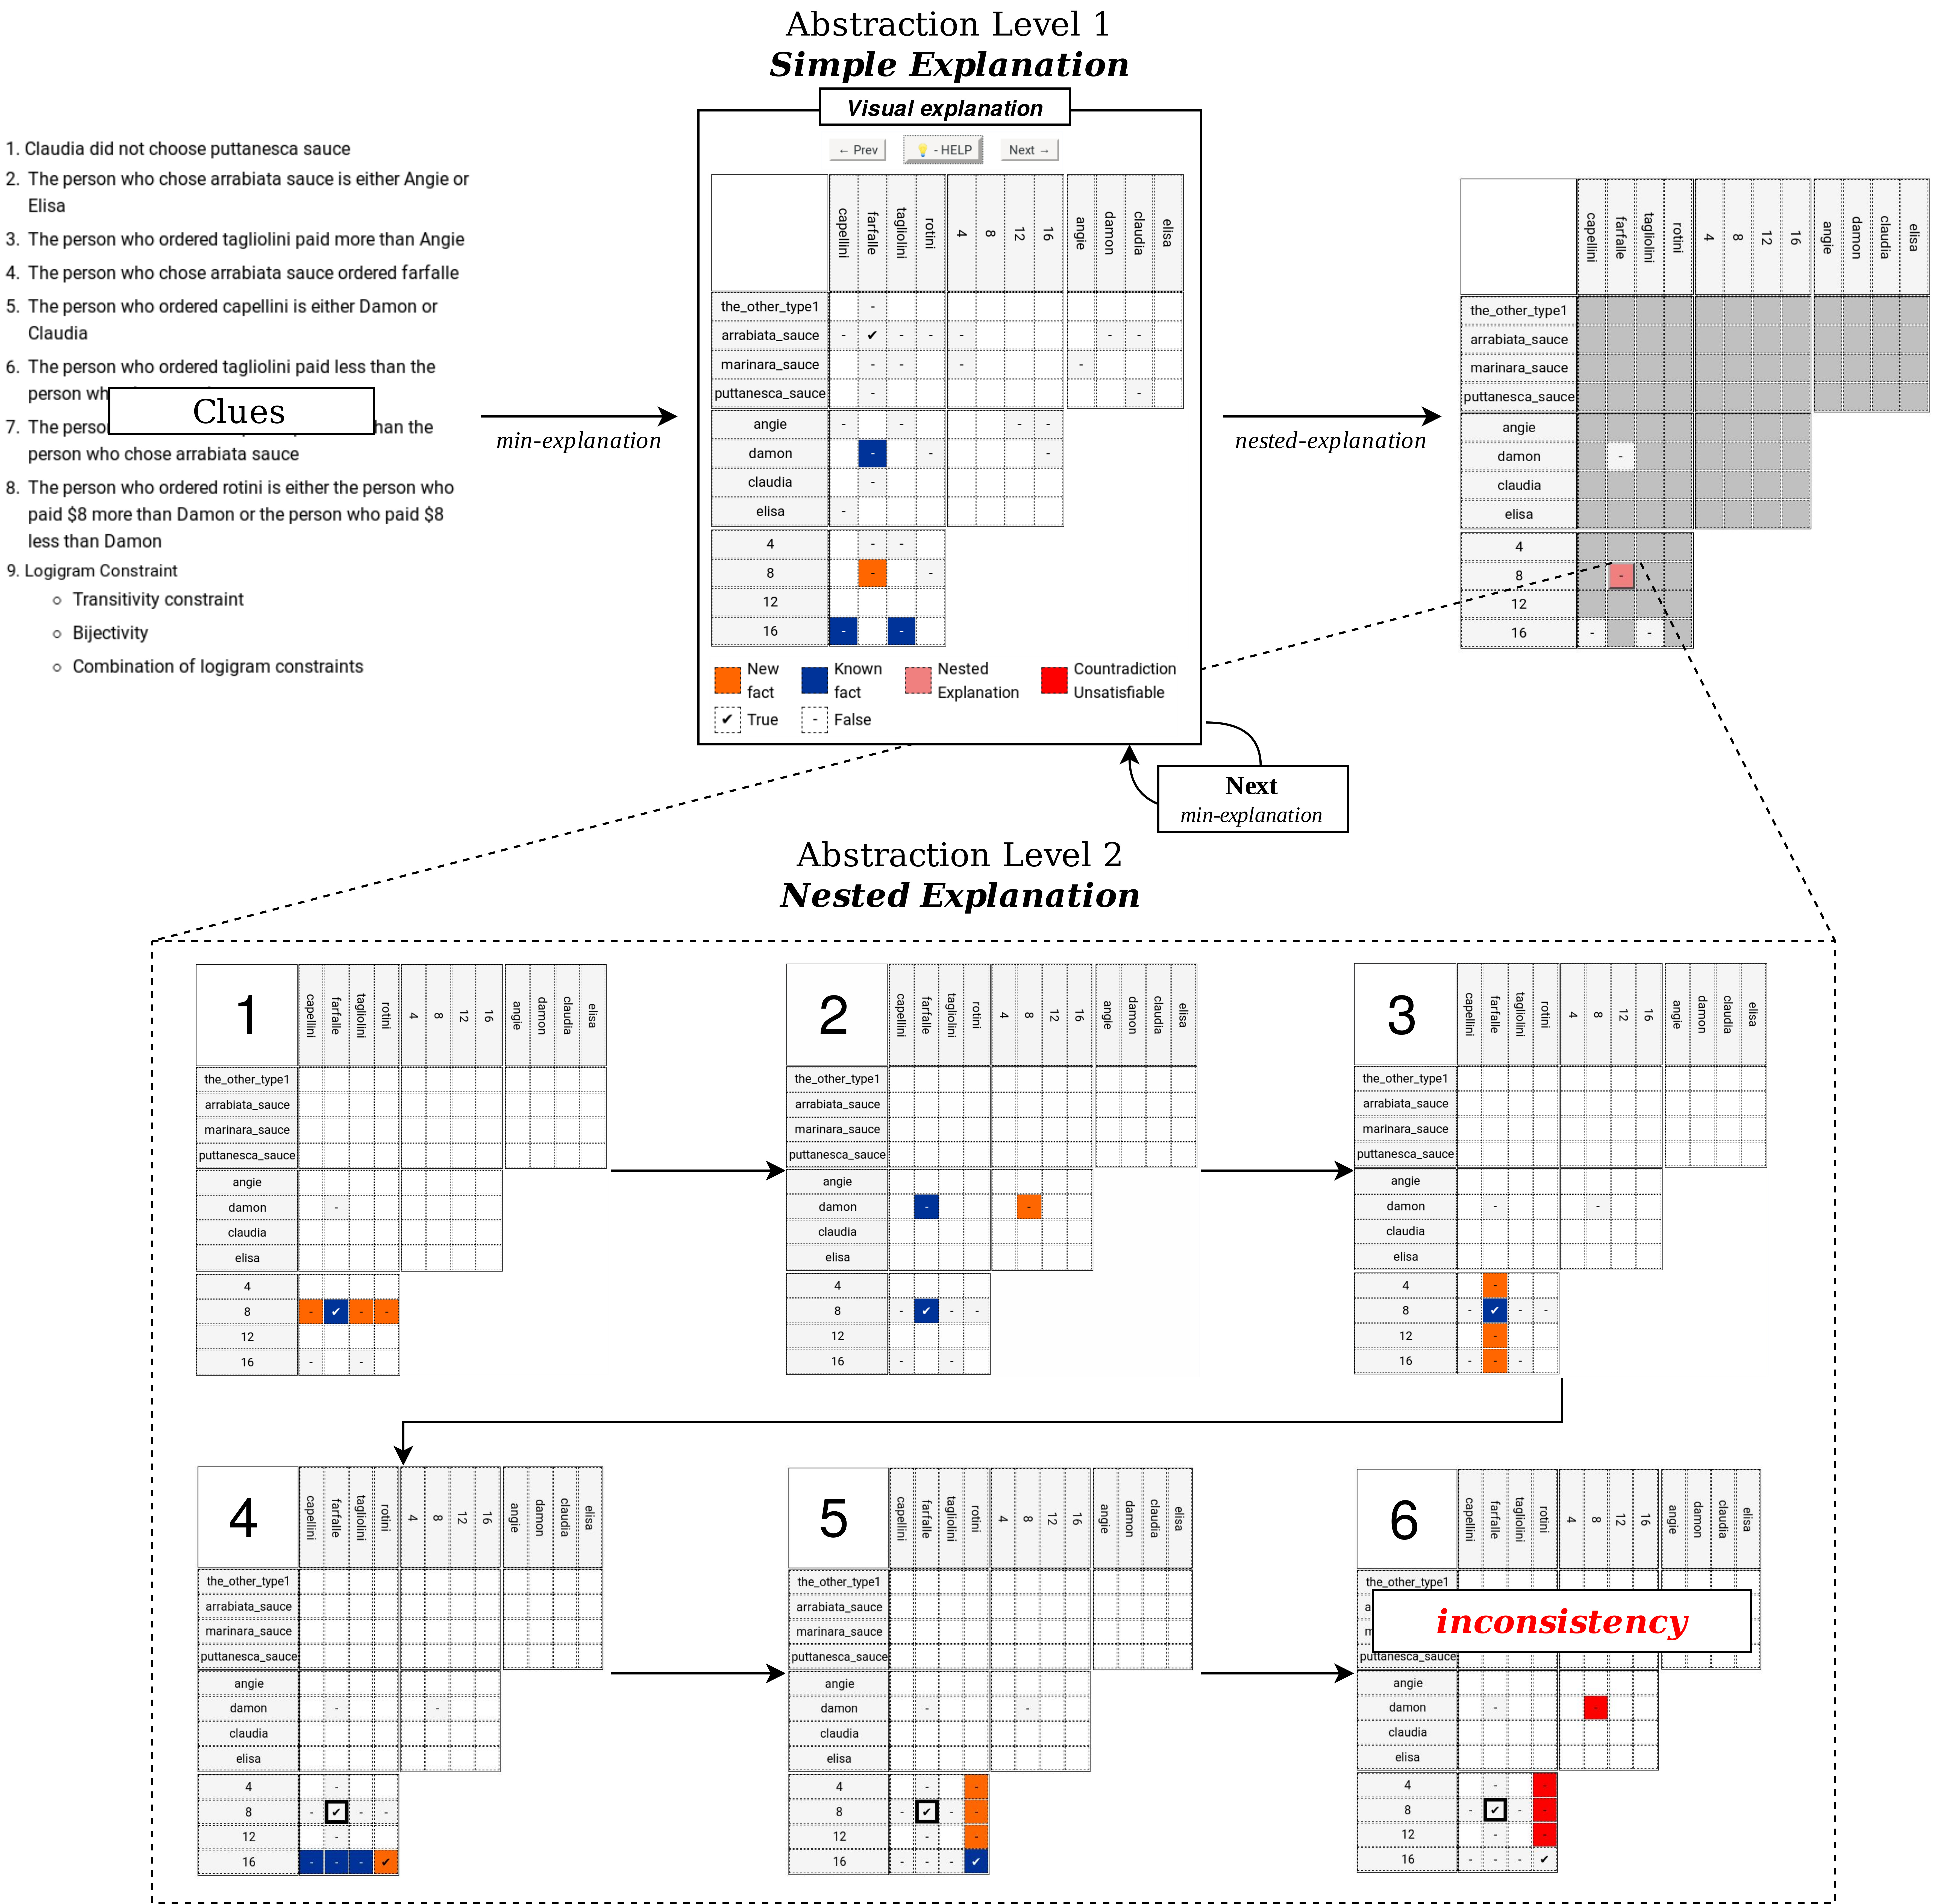
\includegraphics[width=\textwidth]{figures/inconsistency.jpg}
    \caption{A difficult explanation step, including its nested explanation}\label{fig:pasta_diff}
\end{figure}

We hence wish to provide a further, \textit{nested} explanation of such difficult reasoning steps. We believe that an explanation using contradiction is a good tool for this for two reasons: \emph{(i)} it is often used by people when solving puzzles, as well as by mathematicians when proving theorems; and \emph{(ii)} adding the negation of a derived fact such as `Farfalle does not cost \$8', allows us to generate a new sequence of non-redundant explanations up to inconsistency and hence contradiction, hence reusing the techniques from the previous section.
This novel approach allows us to provide a mechanism for \emph{zooming in} into the most difficult explanation step.

\myparagraph{Nested explanation of a reasoning step}

We propose the following principles for what constitutes a meaningful and simple nested explanation, given a non-trivial explanation $(E,S,N)$:
\begin{itemize}
    \item a nested explanation starts from the explaining facts $E$,
          augmented with the counterfactual assumption of a newly derived fact $n \in N$;
    \item at each step, it only uses clues from $S$;
    \item each step is easier to understand (has a strictly lower cost) than the parent explanation with cost $f(E,S,N)$;
    \item from the counterfactual assumption, a contradiction is derived.
\end{itemize}

Note that if an explanation steps derives multiple new facts, e.g. $|N| > 1$, then we can compute a nested explanation for each $n_i \in N$.

More formally, we define the concept of \emph{nested explanation} as follows:

\begin{definition}\label{def:nested-problem}
    The \textbf{nested explanation} problem consists of --- given a non-redundant explanation $(E, S, N)$, and a newly derived fact $n \in N$ --- finding a non-redundant explanation sequence
    \[\langle \ (I_0',(\emptyset,\emptyset,\emptyset)),\ (I_1',(E_1',S_1',N_1')), \dots ,\ (I_n',(E_n',S_n',N_n')) \ \rangle\]
    such that:
    \begin{itemize}
        \item $I_0'$ is the partial interpretation $\{ \neg n_i \wedge E \}$;
        \item $S_i'\subseteq S$ for each $i$;
        \item $f(E_i',S_i',N_i')< f(E, S, N)$ for each $i$;
        \item $I_n'$ is inconsistent; and
        \item a predefined aggregate over the sequence $\left(f(E_i',S_i',N_i')\right)_{i\leq n}$ is minimised.
    \end{itemize}
\end{definition}

We can hence augment each explanation $(E,S,N)$ with a set of nested explanations if they exist. We next discuss algorithms for computing explanations and nested explanations.


\section{Explanation-producing search}\label{sec:expl-gen-prod}
In this section, we tackle the goal of searching for a sequence of $E_i \wedge S_i \rightarrow N_i$ explanations that is as simple to understand as possible, and that ends in the most complete interpretation $I_n$ achievable with the constraints. \tias{terminology of $I_n$, the most complete?} %, e.g. a total interpretation.

Ideally, we could generate all explanations of each fact in $I_n$, and search for the lowest scoring sequence among those explanations. However, the number of explanations for each fact quickly explodes with the number of constraints, and is hence not feasibly to compute. Instead, we will iteratively construct the sequence, by generating candidates for a given partial interpretation and searching for the smallest one among those.

\paragraph{Sequence construction}
We aim to minimize the cost of the explanations of the sequence, measured with an aggregate over individual explanation costs $f(E_i, S_i, N_i)$ for some aggregate like $max()$ or $average()$. The cost function $f$ could for example be a weighted sum of the cardinalities of $E_i$, $S_i$ and $N_i$; see Section~\ref{sec:cost} for the cost function we will use for logic grid puzzles.

Instead of trying to globally optimize the aggregated sequence cost, we encode the knowledge that we are seeking a sequence of small explanations in our algorithm. Namely, we will greedily and incrementally build the sequence, each time searching for the lowest scoring next explanation, given the current partial interpretation. Such an explanation always exist as all facts in the maximally consistent partial interpretation $I_n$ can by definition be derived without search or failure.
%Note that this greedy approach may not find the optimal sequence. 

Algorithm \ref{alg:main} formalizes the greedy construction of the sequence, which determines $I_n$ through propagation and relies on a \textit{min-explanation$(I,C)$} function to find the next cost-minimal explanation. %We assume that the \textit{propagate} function is optimal in that it computes the intersection of all valid solutions, but our approach is also valid for propagation with other levels of consistency.

\begin{algorithm}
%  \begin{algorithmic}
$I_n \gets$ propagate$(\allconstraints)$\;
Seq $\gets$ empty sequence\;
$I \gets \{\}$\;
\While{$I \neq I_n$}{
  $(E, S, N) \gets $min-explanation$(I, \allconstraints)$\;
  append $(E, S, N)$ to Seq\;
  $I \gets I \cup N$
}
% \end{algorithmic}
\caption{High-level greedy sequence-generating algorithm.}
\label{alg:main}
\end{algorithm}

\paragraph{Candidate generation}
$ $\tias{Bart, you had a comment on making this part MUS free. I've made the problem definition MUS free so that a future paper can solve the same problem with non-MUS method}

The main challenge is finding the lowest scoring explanation, among all reasoning steps that can be applied for a given partial interpretation $I$. We first look at how to \textit{enumerate} a set of candidate subset-minimal explanations given a set of constraints.

For a set of constraints $C$, we can first use propagation to get the set of new facts that can be derived from a given partial interpretation $I$ and the constraints $C$. For each new fact $a$ not in $I$, we wish to find a subset-minimal explanation $(E \subseteq I, S \subseteq C)$ that explains $a$.


We hence first find all new facts, and then refine for each fact what a minimal explanation is.

The code below shows our proposed algorithm. The key part of the algorithm is on line \ref{line:mus} where we find an explanation of a single new fact $a$ by searching for a \textit{minimal unsatisfiable core} that includes $\neg a$. We do this over the literals of $I$ as well as over newly introduced \textit{reified} literals for every constraint in $C$. The result will be a minimal unsatisfiable core $\neg a \wedge E \wedge S$ where $E \subseteq I$ and $S \subseteq C$. The latter can in fact be extracted by observing which of the reified literals are set to \textit{true} in the MUS. From $UNSAT(\neg a \wedge E \wedge S)$ we know that $SAT(E \wedge S \rightarrow a)$.

\tias{TODO, integrate MUS part which was higher first}
We will use the concept of Minimal Unsat Cores here (or Minimal Unsat Subset, MUS). A MUS over a set of constraints $C$ is a subset $C' \subseteq C$ such that $C' is UNSAT$ and $\forall c \in C': C' \setminus \{c\} is SAT$. If we know that $N_i$ follows from $S_i$ and $E_i$ then $\neg N_i \wedge S_i \wedge E_i$ must be UNSAT. A Minimal Unsat Subset (MUS) hereof will be a non-redundant subset of $N'_i \subseteq N_i$, $S'_i \subseteq S_I$ and $E'_i \subseteq E_i$ for which we know (because it is UNSAT): $\neg (\neg N'_i \wedge S'_i \wedge E'_i)$ hence through substitution $N'_i \vee \neg (S'_I \wedge E'_i)$ and hence $(S'_I \wedge E'_i) \rightarrow N'_I$. In other words, $(S'_I \wedge E'_i)$ is the smallest explanation of $N'_I$ for which this relation holds, for any smaller explanation it will no longer hold.

We search for minimal unsat cores to avoid redundancy in the explanations. To avoid redundancy at the sequence level, we wish to avoid generating multiple $E \wedge S \rightarrow a, E \wedge S \rightarrow b$ explanations with the same $(E, S)$. Hence, we choose to generate candidate explanations at once for all implicants of $(E, S)$ on line~\ref{line:implicants}. Note that the other implicants $A \setminus \{a\}$ may have simpler explanations that may be found later in the for loop, hence we do not remove them from $J$.

\bart{What is this ``reify'' still doing in the algorithm? } \tias{OK, to remove}
% % \comment{
\begin{algorithm}
% 
\SetKwInOut{Input}{input}\SetKwInOut{Output}{output}
\SetKwComment{command}{/*}{*/}

 \Input{A partial interpretation $I$ and a set of constraints $C$}
% \end{algorithm}
% 
% \Require{$I = $ partial interpretation, $C =$ a set of constraints}
% \Fn(\tcc*[h]{algorithm as a recursive function}){BLA{some args}}{

% \Function{candidate-explanations}{I, C}
  Candidates $\gets \{\}$\;
  $J \gets$ propagate$(I \wedge C)$\;
  $J \gets J \cap I_n$; \textit{\small // only relevant new facts}\\
  \For{$a \in J \setminus I$\label{line:for}}{ 
  \tcp{Minimal expl. of each new fact}
    $X \gets MUS(\neg a \wedge I \wedge C)$ \label{line:mus}\;
    $I' \gets I \cap X$\;
    $C' \gets C \cap X$\;
    $A \gets$ propagate$(I' \wedge C')$; \textit{\small // all implied facts}\label{line:implicants}\\
    add $(I', C', A)$ to Candidates
  }
  \Return{Candidates}
% \EndFunction
\caption{candidate-explanations$(I,C)$}

\label{alg:cand}
\end{algorithm}

% }

\tias{Maak duidelijk dat MUS een keuze is}

We assume the use of a standard MUS algorithm, e.g. that searches for a satisfying solution and if a failure is encountered, the resulting Unsat Core is shrunk to a Minimal Unsat Core~\cite{}. While computing a MUS in this way may be computationally demanding, it is far less demanding than enumerating all MUS's (of arbitrary size) as candidates. 
Hence, the result of the MUS call on line~\ref{line:mus} is \textit{an} unsatisfiable core that is \textit{subset-minimal}, but not \textit{size-minimal}. That is, the unsat core can not be reduced further, but there could be another minimal unsat core whose size is smaller.

%If we want to find the best ordering (TODO), we need the absolute minimal MUS, which is typically only a few constraints.
%This relates to the objective function...

To avoid having te search for all MUS's for each new fact, we use the observation that typically a small (1 to a few) number of constraints is sufficient to explain the reasoning. A small number of constraints is also preferred in terms of easy to understand explanations. We will hence not call \textit{candidate-explanations} with the full set of constraints \allconstraints, but we will iteratively grow the number of constraints used. 
%\bart{ In practice this means that we are doing some form of prioritized explanatoin. 
%First priority: keep the number of constraints small. Second priority, size (which also takes structure into acccount}

\paragraph{Cost functions and cost-minimal explanations}
$ $ \bart{Do we have examples where $A$ is to be taken into account for the size!}  \tias{Not here, but that is the most generic formulation...}
In the following, we assume that we have a cost function $f(I', C', A)$ that returns a score for every possible explanation. The goal will be to find the lowest scoring explanation. We make one further assumption, namely that we have an optimistic estimate $g(C')$ computed on only the constraint part of the explanation, and that $\forall I', A, g(C') \leq f(I', C', A)$. This is for example the case if $f$ is an additive function, such as $f(I', C', A) = f_1(I') + f_2(C') + f_3(A)$ where $g(C') = f_2(C')$ assuming $f_1$ and $f_3$ are always positive.

We can then search for the smallest explanation among the candidates found, by searching among increasingly worse scoring $C'$ as shown in the code below (Algorithm~\ref{alg:minexpl}). This is the algorithm called by the iterative sequence generation (Algorithm \ref{alg:main}).

\begin{algorithm}
\SetKwInOut{Input}{input}\SetKwInOut{Output}{output}
\SetKwComment{command}{/*}{*/}
\SetKw{Break}{break}


 \Input{A partial interpretation $I$ and a set of constraints $C$}
  Candidates $\gets \{\}$\;
  $J \gets$ optimal-propagate$(I \wedge C)$\;
  \For{$C' \subseteq C$ ordered by $g(C')$}{ \label{alg:min:for}
    \If{$g(C') < min(\{f(cand_i) | cand_i \in $Candidates$\})$}{
        \Break\;}
     cand $\gets$ candidate-explanations$(I, C')$\; \label{alg:min:gets}
     add to Candidates all cand$_i$ with corresp. value $f(cand_i)$\;
     }  
          \Return{$cand_i \in$ Candidates with minimal $f(cand_i)$}
 % \EndFunction
\caption{min-explanation$(I,C)$}
\label{alg:minexpl}
\end{algorithm}

Without the optimistic estimate $g()$, we would have to search in the worst case for all possible subsets of constraints. Note that we can cache the \textit{Candidates} set, and in the next iteration we can update the next best candidate $(E, S, N)$ to $(E, S, N \setminus I)$ where $N \setminus I \neq \emptyset$. This candidate now determines a lowerbound to start from \tias{The effect of this could be tried in experimentation}.
Caching of \textit{candidate-explanations()} calls across iterations is not advised as new facts can be used to derive other even newer facts, as well as to provide much simpler explanations for facts that already had an explanation before. These can only be generated by recomputing the explanations again. %are possible, but because the found MUS's need not be cost-minimal, we found that in practice it is better to search for explanations from scratch each time in the hope of finding a cheaper one. \tias{This surely has to be evaluated! It feels naive to me; if no new facts are derived, why do we recompute MUS's for each 'old' fact again and again...} 
\bart{Somewehere (here or in the next section?) we should say something about hte fact that MUS gives us ``just'' a subset-minimal. Without guarantee that it is a good one.
In practice we *do* keep old results...  Becuase they might ``acccidentally'' be  better than new calls... 
I think it fits better in the next section (since it is not conceptual but rather about implementation with the tools we have available}
\tias{OK, will add here}

\textit{Optimization: MARCO map} We identify an additional improvement to the above algorithm, inspired by the MARCO algorithm~\cite{liffiton2013enumerating}. There, they make the observation that given a MUS $M$ involving constraint set $C$, any superset $C''$ of $C$ will also be UNSAT where we already have a corresponding MUS. In our case, given that we search candidate explanations for an increasingly costly constraint set $C$, if we have a candidate explanation involving $C'$ on line \ref{alg:min:gets} we can omit searching for explanations of $C'' \supset C'$ in the for loop on line \ref{alg:min:for}, as an explanation involving $C''$ would have $g(C'') > g(C')$. \tias{actually, there could be a smaller one than $C'$ which is found when searching for a MUS of $C''$ but we leave that detail open here}.
\tias{Future idea: if a constraint is fully satisfied, no need to include it in future calls. I guess because the 'propagate' will return empty the overhead is quite limited anyway}
\bart{There might be some overhead. THe reason is that in that theory also all the implicit constraints are. In practice they propagate the same for every satisfied clue... } 
\tias{OK, so we should try empirically but don't have the time now}




%\textbf{That is it for now... more optimisations are possible, basically in the way we search over the C', like, cache Candidates so that its minimum value is maintained (and do an 'update' to it before starting to potentially clean it); do not search for $C'' \supset C'$ where C' has some explanations; perhaps we can find out that at some point we no longer need to optimalprop some $C'$? (e.g. a 'fully used' clue?)}



\section{Explanations for logic grid puzzles}\label{sec:zebra}
We instantiated the above described algorithm in the context of logic grid puzzles. 
In that setting there are basically three types of constraints in $\allconstraints$: transitivity constraints, bijectivity constraints and clues, where the first two follow the same structure in every puzzle and the clues are obtained in a mostly automatic way (see Section \ref{sec:holistic}). 
Before defining a cost-function, and the estimation for $g$ used in our implementation, we provide some observations that drove our design decision. 

\paragraph{Observation 1: Propagations from a single implicit constraint are very easy to understand} Contrary to the clues, the implicit constraints (transitivity/bijectivity) are very limited in form and propagations over them follow well-specified patterns. 
For instance in the case of bijectivity, a typical pattern that occurs is that when $X-1$ out of $X$ possible values for a given function have been derived not to be possible, it is propagated that the last value should be true; this is visualized for instance in Figure \ref{fig:zebrascreen}. 
Hence, in our implementation, we ensure that they are always performed first. Stated differently, $g$ and $f$ are designed in such a way that $g(S_1)\geq f(I,S_2)$ whenever $S_2$ consists of only one implicit constraint and $S_1$ does not. 

\paragraph{Observation 2: Clues propagate rarely by themselves}
We observed that the automatically obtained logic representation of clues usually has quite weak (unit) propagation strength in isolation. 
This is not a property of the clues, but rather of the final obtained translation. As an example, consider the following sentence: 
``The person who ordered capellini is either Damon or Claudia''. From this, a human reasoner might conclude that Angie did not order capellini. 
% The use of the article ``the'' in the above sentence gives away that there is actually a unique person who ordered capellini. 
However, the (automatically) obtained logical representation is 
\[\exists p\in \mathit{person}: \mathit{ordered}(p, \mathit{capellini})\land (p =  \mathit{Damon}\lor p =  \mathit{Claudia}).\]
This logic sentence only entails that Angie did not order capellini \emph{in conjunction with the bijectivity constraint on $ \mathit{ordered}$}.
In the natural language sentence, this bijectivity is implicit by the use of the article ``The'' which entails that there is a unique person who ordered capellini. 

We observed that there is rarely any propagation from sole clues, and that only few implicit constraints are active together with a clue at any time. Hence, when pairing clues to other constraints we always pair it with the set of all implicit (bijectivity, transitivity) constraints.
\bart{This last sentence is unclear... 
Drop or CHange to??? ``Because of this last observation, in our implementation for logic grid puzzles we decided not to consider all subsets of implicit constraints in combination with a clue as candidate sets $S$ in Line \ref{alg:min:for} in Algorithm \ref{alg:minexpl} but instead combine the set of all implicit constraints, subsequently counting on the non-redundance (the subset-minimality of the core) to eliminate most of the implicit constraints since they are not used anyway. }

\paragraph{Observation 3: Clues are typically used independently from other clues} 
A next observation is that in all the puzzles we encountered, human reasoners never needed to combine two clues in order to derive new information and that when such propagations are possible, they are quite hard to explain, and can be split up into derivations containing only single clues.
The latter is of course not guaranteed, since one can artificially devise disjunctive clues that do not allow propagation by themselves. 
Our algorithms are built to handle this case as well, but it turned out to be not necessary in practice: in the puzzles we tested, we never encountered an explanation step that combined multiple clues. 

\paragraph{Observation 4: Previously derived facts are easier to use than clues or implicit constraints}
Our final observation that drove the design of the cost functions is that using previously derived facts is often easier than using an extra clue or implicit constraint. This might be due to the fact that previously derived facts are of a very simple nature while, even implicit constraints contain quantification and are thus harder to grasp. An additional reason for this perceived simplicity is that the derived facts are visualized in the grid. 


\paragraph{A cost function}
With these three observations in mind, we devised $f$ and $g$ as follows (where $nc(C)$ denotes the number of clues in $C$): \label{sec:cost}
\begin{align*}&f(I,C) = basecost(C) + |I| + 5\cdot|C|\\
&g(C) = basecost(C) = \left\{\begin{array}{ll}
                               0 & \text{if $|C|=1$ and $nc(C) = 0$}\\
                               20 & \text{if $|C|>1$ and $nc(C)=0$}\\
                               20\cdot nc(C) & \text{otherwise}
                              \end{array}\right.
                              \end{align*}
                              
The number $20$ is taken here to be larger than any reasonable explanation size. 
\bart{Due to the factor 5 the 20 is no longer ''larger than any reasonable size... Emilio, can you increase this to 100? }
The effect of this,  is that we can generate our subsets $S$ in Line \ref{alg:min:for}
 of Algorithm \ref{alg:minexpl} in the following order:
\begin{itemize}
 \item First all $S$ containing exactly one implicit constraint.
 \item Next, all $S$ containing exactly all implicit constraints and (optionally) exactly one clue.
 \item Finally, all clue pairs, triples etc. though in practice this is never reached.
\end{itemize}
Summarized, our instantiation for logic grid puzzles differs from the generic methods developed in the previous section in that it uses a domain-specific optimization function $f$ and does not considering all $S$ in Line \ref{alg:min:for}, but only promising candidates based on our observations.

For the complete non-redundant explanation sequence our tool produces on the running example using these scoring functions, we refer to \url{http://bartbog.github.io/zebra/pasta}. An example of the hardest derivation we encountered (with cost 28\bart{TODO COST!}), as well as its nested explanation, is depicted in Figure \ref{fig:pasta_diff}. It uses several bijectivity constraints for uniqueness of persons, but also for reasoning on the relation between costs and types of pasta, in combination with a clue and three assumptions.

When investigating the nested explanation produced by the system, one can observe that this explanation does not entirely match an explanation that would be produced by a human reasoner for a couple of reasons: 
\begin{itemize}
 \item In the generation of the nested explanation, as well is in the high-level sequence, we used the greedy algorithm from the previous section. While at the high level, this yields good results, at the nested level, this results in sometimes propagating facts that are not used afterwards. The very first propagation in the nested explanation of this kind. While this would be easy to fix by postprocessing the generated explanation, we left in our example to highlight this difference between the nested and non-nested explanation. 
 \item It sometimes happens that the system finds, as a minimal explanation on in which $X-1$ negative facts are used instead of the corresponding single positive fact. This can be seen in the last step. For human reasoners the positive facts often seem to be easier to grasp. A preference for the system towards these negative facts might be incidentally due to formulation of the clues or it can incidentally happen due to the way the MUS is computed (only subset-minimality is guaranteed there). 
 In general, observations of this kind should be taken into account when devising a cost function.  
\end{itemize}



\ignore{
\begin{figure}[ht]
\centering
\includegraphics[width=\linewidth]{figures/zebra_screen_2}
\caption{Demonstration of hard explanation.}
\label{fig:screen2}
\end{figure}
\bart{Screenshot quality}


Intuitively, the reasoning happening here can be explained as follows: if \textit{farfalle} were to cost \$8, then due to the assumptions and bijectivity \textit{rotini} would cost 16. However, since Damon did not take \textit{farfelle} (which we assumed costs \$8), this is in contradiction with the highlighted clue. Hence \textit{farfalle} does not cost \$8. 
}



\section{Logic grid puzzles: From natural language clues to typed first-order logic}\label{sec:holistic}
% Description of our pipeline, including the NLP part (though not fully automated):
% Can include Jens' table on challenges for BOS even with fully correct lexicon (from his poster).
% TODO : add ZebraTutor in Latex logic Mode
We developed a demo system which is an integrated solution for solving logic grid puzzles, and for explaining in a human-understandable way how the solution can be obtained from the clues. 

The input to ZebraTutor is a plain English language representation of the clues and a list of all the \textit{entities} present in the puzzle. It then applies NLP techniques to build a puzzle-specific lexicon. This lexicon is fed into a type-aware variant of the semantical framework of Blackburn \& Bos, which translates the clues into Discourse Representation Theory. The logic is further transformed to a specification in the IDP language, a typed extension of first-order logic. 

The underlying solver, IDP\cite{pip:de2018predicate} uses this formal representation of the clues both to solve the puzzle and to explain the solution. 

% Pipeline description of the steps form start to end
\paragraph{Steps} Our framework consists of the following steps, starting from the input:
\begin{enumerate}\setlength\itemsep{-0.2em}
	\item[A] Part-Of-Speech (POS) tagging: A part-of-speech tag is associated with each word using an out-of-the-box PoS tagger.\\
	\item[B] Chunking and lexicon building: A problem-specific lexicon needs to be constructed. In the lexicon, each word or set of words (chunk) is assigned a role, based on the POS tags. Based on these roles, we have identified a grammar in the Blackburn and Bos framework for interpreting clues of logic grid puzzles. The grammar was created based on 10 example training puzzles, and evaluation on 10 different test puzzles showed that it could also cover these cases..\\
	\item[C] We use a typed variant of the Blackburn and Bos semantic framework to use the lexicon and grammar to derive a logical formulation of the clues in Discourse Representation Theory. The typed extension allows us to discover the case where different verbs are used as synonyms for the same inherent relation between two types, e.g. 'lives in(person, house)' and 'owns(person, house)'. The typed discourse representation theory is then translated into IDP language and the bijectivity and transitivity constraints are automatically added. \\
	\item[D] Explanation-producing search in IDP: this is the main contribution of this paper, as explained in Section~\ref{sec:expl-gen-prod}.\\
	\item[E] Visualisation of the explanation: the $(E_i, S_i, N_i)$ explanations are visualized by means of a color-coded logic grid, where different colors are used to highlight the $E_i$ and $N_i$ cells, and where the constraints of $S_i$ are highlighted as well. Figure~\tias{TODO} shows an example. An online demo can be seen on \url{http://bartbog.github.io/zebra}. \tias{Check that it is not a blind submission!!!!}
\end{enumerate}

A more detailed explanation of steps B and C of the information pipeline can be found in \cite{mcs:claesuser}. From a natural language processing point of view, the most difficult part is step B: automatically deriving the right lexicon. In our current system, this is a semi-automated method that suggests a lexicon and lets a user modify and approve it once. The reason is two fold: 1) the current approach assumes the clues are written in controlled natural language that abides to the (generic) grammar rules. However, puzzle developers are often keen to craft seeming ambiguities (reusing a verb for two relations, name ambiguations, use of gender to discriminate names), or add unnecessary words or contextual synonyms (in the morning, when there is only one timeslot before 12:00). In those case, the user has to reformulate those sentences into the unambiguous controlled natural language. Reason 2) is that our explanation generation step assumes a consistent theory. If one of the clues is missing or wrong, it would be unable to completely solve the puzzle as the resulting $I_n$ would not match the intended puzzle solution.

%The first three steps are related to Natural Language Processing and are discussed in subsection \ref{nlp}.%Step C is explained in subsection \ref{idp_spec}.
%
%Steps D and E describe the explanation-generating search for solving the puzzle imitating the human train-of-thought.
%
%\subsection{Natural Language Processing} \label{nlp}
%The standard procedure in Natural Language Processing is to start by tagging each word with its estimated Part-Of-Speech tag (POS tag). 
%
%\subsubsection*{Step A. Part-Of-Speech (POS) tagging} \label{pos_tagging}
%We use the standard English Penn Treebank II POS tagset \cite{marcus1993building}. As POS tagger we use NLTK's built-in Perceptron tagger \footnote{\url{http://www.nltk.org}}. It uses a statistical inference mechanism, trained on a standard training set from the Wall Street Journal. Since any POS-tagger can make mistakes, we ensure that all of the puzzle’s entities are tagged as noun.
%
%\subsubsection*{Step B. Chunking and lexicon building} \label{chunking_lexicon}
%To use the extended Blackburn \& Bos framework, a lexicon and grammar have to be provided, where the lexicon assigns a role to different sets of words and the grammar is a set of rules describing how words can be combined into sentences. The grammar is constructed for logic grid puzzles in general and not puzzle specific; the lexicon is partly problem-specific and partly problem-agnostic.\\
%
%Thus, the goal of this second step, called chunking, is to group POS-tagged words into chunks to form a lexicon. Each chunk is associated with a (puzzle-specific or general) lexical category\footnote{The 3 \textbf{puzzle specific} lexical categories are \textit{proper nouns}, namely the individual entities that are central to the puzzle, \textit{other nouns} that refer to groups of entities (like house, animal) and \textit{transitive verbs} that link two entities to each other; the other categories are general and contain a built-in list of possible members. The categories are \textit{determiner},\textit{ number, preposition, auxiliary verb, copular verb, comparative} and \textit{some*}-words (somewhat, sometime, ...), and \textit{conjunction}.} introduced by Claes \cite{msc/Claes17}. We use NLTK and a custom set of regular expressions for chunking the proper nouns and different types of transitive verbs.\\ 
%
%The automatically generated lexicon is verified in order to make sure that the clues can be transformed into a complete IDP specification of the puzzle problem in the subsequent step.
%
%\subsubsection*{Step C. From chunked sentences to a complete IDP specification} \label{chunked_to_logic}
%
%
%\subsection{Explaining Logic Grid Puzzles} \label{explaining_puzzles}
%Based on the previously built idp specification of a puzzle, we use the idp system to solve the problem using an (human-like) explanation-generating search.
%
%\subsubsection*{Step D. Explanation-generating search in IDP} \label{idp_search}
%
%
%\subsubsection*{Step E. Visualisation of the explanation} \label{visualisation_explanation}
%We have explored two different possibilities to present the explanations to humans. The first was generating natural language sentences of the form "From the clue(s) $\langle$clue$\rangle$, and the fact that $\langle$assumptions$\rangle$, it follows that $\langle$conclusions$\rangle$." Overall we were not satisfied with the outcome of the generated sentences. As soon as there are a couple assumptions, this kind of sentence easily becomes hard to read and understand. As a result, we have decided to use of the standard grid in logic puzzles. For each step, we highlight which clue(s) are used, all cells used for the propagation in blue and all conclusions in orange.
%
%\section{Demonstration}
%Figure 1 contains a screenshot of this explanation process. It displays a partially filled grid, in which check-marks represent that something is derived to be true and minus signs that it is false. The working of our system is demonstrated on http://bartbog.github.io/ze

\section{Experiments}\label{sec:experiments}
The explanation-generating search has been tested against unseen puzzles on a computer with the following specifications:

\begin{table}
	\centering
	\resizebox{0.8\columnwidth}{!}{%
		\begin{tabular}{|l|l|l|l|}
			\hline 
			CPU & CPU Freq. & cores & RAM Size \\ 
			\hline 
			Intel(R) Xeon(R) CPU E3-1225 & 3.30 GHz & 4 & 32 Gb \\ 
			\hline 
		\end{tabular} 
	}
\caption{Computer system specifications}
\label{table:system_specifications}
\end{table}

We analyze the results in 3 directions :

\paragraph{Q1. How do different puzzles compare with respect to the generated explanations ?} For future reference, we denote \textbf{c} = $c_1, c2, ...c_n$ the costs, where $c_i$ is the cost, based on the cost function $f(I, C)$, at reasoning step $i$ and n the number of reasoning steps to solve a problem. Table \ref{table:sequence_leve} shows how difficult the puzzles are by means of the total cost and how the expensive a new conclusion is based on the current state of the grid.

\begin{table}
	\centering
	\resizebox{\columnwidth}{!}{%
\begin{tabular}{|c||c|c|c|c|c||c|c|c|c|c|c|} 
\hline 
\textbf{Puzzle} & \textbf{n} & $\sum_{i = 1}^{n} c_i$  & max(\textbf{c}) & $\overline{\text{\textbf{c}}}$ & \textbf{5 Highest costs} & \textbf{\% bij.} & \textbf{\% trans.} & \textbf{\% comb.} & \textbf{\% clue} & \textbf{\% multi. clues} \\ 
\hline 
p5 & 113 & 626 & 25 & 5.59 & [25, 21, 21, 21, 21] & 31.0 & 50.0 & 0 & 19.0 & 0 \\ 
\hline 
p16 & 122 & 680 & 23 & 5.62 & [23, 21, 21, 21, 21] & 21.0 & 60.0 & 0 & 19.0 & 0 \\ 
\hline 
p93 & 119 & 659 & 21 & 5.58 & [21, 21, 21, 21, 20] & 34.0 & 47.0 & 0 & 19.0 & 0 \\ 
\hline 
p12 & 115 & 591 & 23 & 5.18 & [23, 21, 21, 21, 20] & 29.0 & 54.0 & 0 & 17.0 & 0 \\ 
\hline 
p18 & 116 & 615 & 22 & 5.35 & [22, 22, 22, 21, 21] & 28.0 & 55.0 & 0 & 17.0 & 0 \\ 
\hline 
p20 & 116 & 552 & 22 & 4.8 & [22, 21, 21, 21, 20] & 27.0 & 58.0 & 0 & 15.0 & 0 \\ 
\hline 
p25 & 111 & 595 & 24 & 5.41 & [24, 23, 22, 21, 21] & 37.0 & 45.0 & 0 & 17.0 & 0 \\ 
\hline 
p19 & 123 & 630 & 22 & 5.16 & [22, 21, 21, 21, 21] & 25.0 & 59.0 & 0 & 16.0 & 0 \\ 
\hline
\end{tabular} 
	}
\caption{Puzzle explanation cost based on the cost function $f(I, C)$ and statistics on puzzle constraints}
\label{table:sequence_leve}
\end{table}

While the first part of the table \ref{table:sequence_leve} only analyzes the difficulty of a puzzle, the second part focuses on the explanations. 
Most of the explanations are either generated using bijectivity (bij.) or Transitivity (trans.). The rest are found using the 1 or more clues, or by combining (comb.) transitivity with bijectivity. This is due to the way puzzles are formulated in natural language for logic grid puzzles.

\paragraph{Q2. How does the level of difficulty progress throughout the explanation?} bla bla bla

% TODO graph : 

\paragraph{Q3. How is the performance and the level of difficulty affected by removing parts of the algorithm ? } bla bla bla

% TODO table : Leaving some parts of the algo out, to see step-wise improvements of the components?  Some experiment with different levels of abstraction (e.g. all constraints at once, clues separate but all implicit at once, 2 groups of implicits, full split of implicits) with 'set of measures', so probably a table

\paragraph{Bonus. How well does it compare to human solving process ?} 

% TODO Compare with the tutorial puzzle of logicgridpuzzles.com? Ideally, a small human evaluation (e.g. ask people to solve a 3-with-3 puzzle and note the order of derivations and clues used, compare this 'ranking' to our ranking, discuss some differences.



\section{Discussion, future work, and conclusions}\label{sec:conclusion}
In this paper, we formally defined the problem of step-wise explanation generation and presented a generic algorithm for solving this problem. 
We implemented this algorithm in the context of logic grid puzzles, where we start from natural language clues and provide a human-friendly explanation in the form of a visualisation.
We used this implementation to investigate puzzle properties and difficulty. 

The main bottleneck of the current algorithm is the many calls to MUS, which is a hard problem by itself. 
Therefore, in future work we want to investigate unsat-core \emph{optimization} with respect to a cost-function, either by taking inspiration for instance from the MARCO algorithm~\cite{liffiton2013enumerating} but adapting it to prune based on cost-functions instead of subset-minimality, or alternatively by reduction to QBF \cite{QBF}.

Secondly, we want to dig deeper into the question \emph{what constitutes an understandable explanations for humans}, either by optimizing the entire sequence instead of step by step, by learning the cost function based on user traces, or by reusing our developed algorithms to explain reasoning steps in more detail and as such develop an explanation mechanism that operates at different levels of abstraction. 
To illustrate this last point: in the setting of very difficult puzzles, some of the explanation steps still require some effort to understand. 
When explained by a human, this is often done using some form of proof by contradiction using an explanation of the form ``suppose this [the derived fact] would not hold, then [some simpler reasoning steps], which is not possible''. This is also how we explained Figure \ref{fig:screen2} at the end of Section \ref{sec:zebra}.
This explanation process is of \emph{exactly the same form} as what we generate now. The only difference is that $I_0$ is not the empty interpretation, but one in which a wrong value is assigned. 

A final direction for future work is to make our approach interactive, essentially allowing \ourtool to be called \emph{while} a user is solving the puzzle and to implement in more serious domains such as for instance interactive configuration in which a human and a search engine cooperate to solve some configuration problem and the human can often be interested in understanding \emph{why} the system did certain derivations \cite{DBLP:journals/tplp/HertumDJD17,DBLP:conf/bnaic/CarbonnelleADVD19}. 


% \section*{Author Contributions}
% \bart{Is this required? Where does this come from? 

% If it is, I like the second style more. Also, We should Acknowledge Jens's work indeed, but probably rather in the Acknowledgement section}


% \todo{Please add anything relevant, i don't remember who did what specifically}
% \emilio{e.g All authors contributed equally to the writing of the paper?}

% \noindent\textbf{Bart Bogaerts} helped with the \textit{Software}, the \textit{Visualisation} and \textit{Writing} of the paper.

% \noindent\textbf{Emilio Gamba} helped with the \textit{Visualisation}, the \textit{Experiments}, and the \textit{Writing} of the paper.

% \noindent\textbf{Tias Guns} helped with \textit{Conceptualisation} of the research and experiments, \textit{Supervision} and the \textit{Writing} of the paper.

% \tias{or something like (maybe Bart wants to add something more? smth like grateful to Jens for system describe din Sec 8?):} BB and TG conceived the research, BB and EG implemented the software, EG performed the experiments and all authors contributed equally to the design of the experiments and the writing of the paper. \tias{First time I have to do this}

\section*{Acknowledgements}
This research received funding from the Flemish Government under the ``Onderzoeksprogramma Artifici\"ele Intelligentie (AI) Vlaanderen'' programme. 
We thank Jens Claes (and his master thesis supervisor Marc Denecker) for the implementation of a typed extension of the Blackburn \& Bos framework as part of his master's thesis, as well as Rocsildes Canoy for his help with the NLP aspect of the information pipeline. %\todo{Thank Jens (and Rocs?) (and co-supervisors of Jens' thesis?)}

% \section*{References}

\bibliography{mybibfile,ref,krrlib}

\end{document}
